\documentclass[11pt, a4paper, USenglish]{article} % change ``USenglish'' to ``norsk'' if applicable.
\usepackage{tabstackengine}
\stackMath
\usepackage{kyblab} % Contains all included packages. See kyblab.sty.
\usepackage[framed,numbered,autolinebreaks,useliterate]{mcode}
\usepackage{textcomp}
\addbibresource{bibliography.bib} % Makes the bibliography file available to biblatex.
\newcommand{\td}[1]{\dot{\tilde{#1}}}
\newcommand{\tdd}[1]{\ddot{\tilde{#1}}}
\newcommand{\MATLAB}{\textsc{Matlab}\xspace}
\begin{document}

% Titlepage
\title{LaTeX Lab Report Template}
\author{Group 16\\Odin Aleksander Severinsen\\Sigurd Totland\\Viktor Korsnes}
\date{\today}
\begin{titlepage}
    \maketitle
    \begin{figure}
    \centering
    
\includegraphics[width=0.5\textwidth]{figures/itk_ntnu}\\
    Department of Engineering Cybernetics
    \end{figure}
    \thispagestyle{empty}
\end{titlepage}

% Abstract
\newpage
\begin{abstract} 
%\addcontentsline{toc}{section}{Abstract} % add this if you want the abstract in the table of contents.
  In this this project a physical helicopter model is controlled using different methods to obtain stability and easy controllability with a joystick. The control methods are all based on a linearized mathematical model of the system. Among them are feed forward control, monovariable feedback control, and feedback control using a linear quadratic regulator (LQR). The latter was done both with direct state feedback and with state estimation using a linear observer. 
\end{abstract}

\thispagestyle{empty} % Avoid page numbering on the abstract page.

% TOC
\newpage
\tableofcontents
\thispagestyle{empty} % Avoid page numbering on the table of contents.

% Main content
\newpage
\setcounter{page}{1}
\section{Introduction}\label{sec:intro}
Your introduction should contain an overview of the work you were assigned, as well as a few sentences putting the work into a larger perspective. You should also give a quick description of how the report is organized (as is done below).

You should of course put most of the work into doing good work in the lab and then presenting it in the report. When presenting your work in the report, both content and presentation/layout matters. Since your only way of communicating your good effort in the lab is through writing about it here, the way you write about it is essential. This means that even if you have the very best controller but describe it poorly, you will probably not be rewarded for the good results. A plot showing perfect control is worth very little if it is not accompanied by a clear description of what it represents.

Layout is naturally less important than content, but it still matters. You can think of report writing like selling an apartment; when you present your apartment for potential buyers you will of course clean the apartment and make it good looking. How clean the apartment is does of course not determine its value, but it is still important since it influences the subjective value your buyers will put on the apartment. 

\subsection{Software}
You are of course free to use whatever software you want for report writing. You can also submit a handwritten report, although this is probably not a great idea if your handwriting can be hard to read. 

You can also use Word or a similar word processor. However, it is next to impossible to achieve decent layout with Word. The support for vector graphics (discussed later) is extremely poor, and text tends to look pretty bad (bad support for kerning and ligatures). Furthermore, math is both time consuming and difficult to input, and tends to look very ugly. In general, a report written in Word looks like a draft.

It is strongly recommended to use Latex. Unless you tweak the layout too much, your report will almost certainly look very good. Although it can take a bit of effort to get started, it is also much quicker to use than Word and similar programs. The support for math and vector graphics is also great.

If you are new to Latex, you can have a look at the source for this document to get started. You can also look at the presentation by~\cite{Berland2010} (in Norwegian) or consult~\cite{Oetiker2011}. Another good reason to learn Latex is that you probably don't want to write your master's thesis in something like Word, doing so would likely be very frustrating. Being reasonably fluent in Latex before you get that far will make your thesis work much smoother.

Some of you are probably fluent in Latex and might plan to write the report using it. Please resist the temptation (if any) to change the fonts, make super fancy headers (they are not necessary for a report like this), change the margins, change the paragraph indentation and/or spacing, and similar things.

A great tool for collaborating on Latex documents is ShareLaTeX at \url{https://www.sharelatex.com/}; if you use this you won't have to install anything on your computer. Texmaker at \url{http://www.xm1math.net/texmaker/} is a good cross-platform editor. Some people like Lyx, which is a Latex editor that behaves a little bit like Word. If you prefer to compile your Latex document on the command line, the latexmk \url{https://www.ctan.org/pkg/latexmk} command is a great tool included in most TeX distributions. There is also a simple Vim plugin that uses latexmk as its backend called LaTeX-BoX \url{https://github.com/LaTeX-Box-Team/LaTeX-Box}.

\subsection{Other Comments}
Unless you have a very good reason not to, you should write the report in English. If you have problems with Latex, the solution is usually just a few Google searches away.

This report is organized as follows: \Cref{sec:prob_descr} contains some course specific equations, and some tips on how to create illustrations. Several \LaTeX{} tips can be found in \Cref{sec:latex_tips}, such as how to create a table and matrix equations. \Cref{sec:figures} contains some advice on using plots from MATLAB\@. The closing remarks are in~\Cref{sec:conclusion}, respectively. \Cref{sec:matlab} contains a MATLAB file while \Cref{sec:simulink} shows an example Simulink diagram. The Bibliography can be found at the end, on page~\pageref{sec:bibliography}.

\section{Problem Description}\label{sec:prob_descr}
The problems revolves around a physical system of a helicopter arm which is fasten to the ground and has three degrees of freedom. Elevation ($e$), pitch ($p$) and travel ($\lambda$). 
The helicopter was controlled through a joystick and interfaced to the helicopter with \MATLAB. The following tasks are described in the report:

\begin{itemize}
    \item Derive a mathematical model for the system.
    \item Derive and apply PD and multivariable controllers for the system.
    \item Estimate states that are not directly measured.
    \item Develop a linear quadratic regulator (LQR) for the system.
\end{itemize}

The helicopter can be modeled as three point masses: two masses represent the motors of the propellers and the third is the counterweight on the opposite side. Refer to figure~\ref{fig:heli} for depiction of setup. The cynlindres of figure~\ref{fig:heli} are the joints where the axis of the cylindres are equal to the axis of rotation of the joint. The following definitions are made: \textit{p} is the pitch angle of the helicopter head, \textit{e} is denotes its elevation angle and \textit{$\lambda$} denotes the travel angle of the helicopter. Figure \ref{fig:heli} shows all angles at zero and with positive orientation as indicated. For the sake of this report, it is assumed that there is a linear relationship between the forces the propellers generate and the voltage that is applied to them:

\begin{subequations}\label{eq:P1_forces_propellers}
    \begin{align}
        F_f&=K_f V_f     \label{eq:P1_forces_propellers_f} \\
        F_b&=K_b V_b     \label{eq:P1_forces_propellers_b}
    \end{align}
\end{subequations}

The propellers are placed symmetrically in relation to the pitch axis and the forces always attack perpendicular to the plane made by the pitch and elevation axis. The weight of the the point masses are called $F_{g,f}, F_{g,b}$ and $F_{g,c}$ and attack parallel to gravity.

For the sake of this report, it is assumed that the weight of the two propeller motors are equal and given by $m_p$. The counterweight mass is indicated by $m_c$. The distance along the elevation axis between the travel axis and pitch axis is indicated by $l_h$. The length from the travel axis to the counterweight is indicated by $l_c$. 

\begin{figure}[bp]
	\centering
	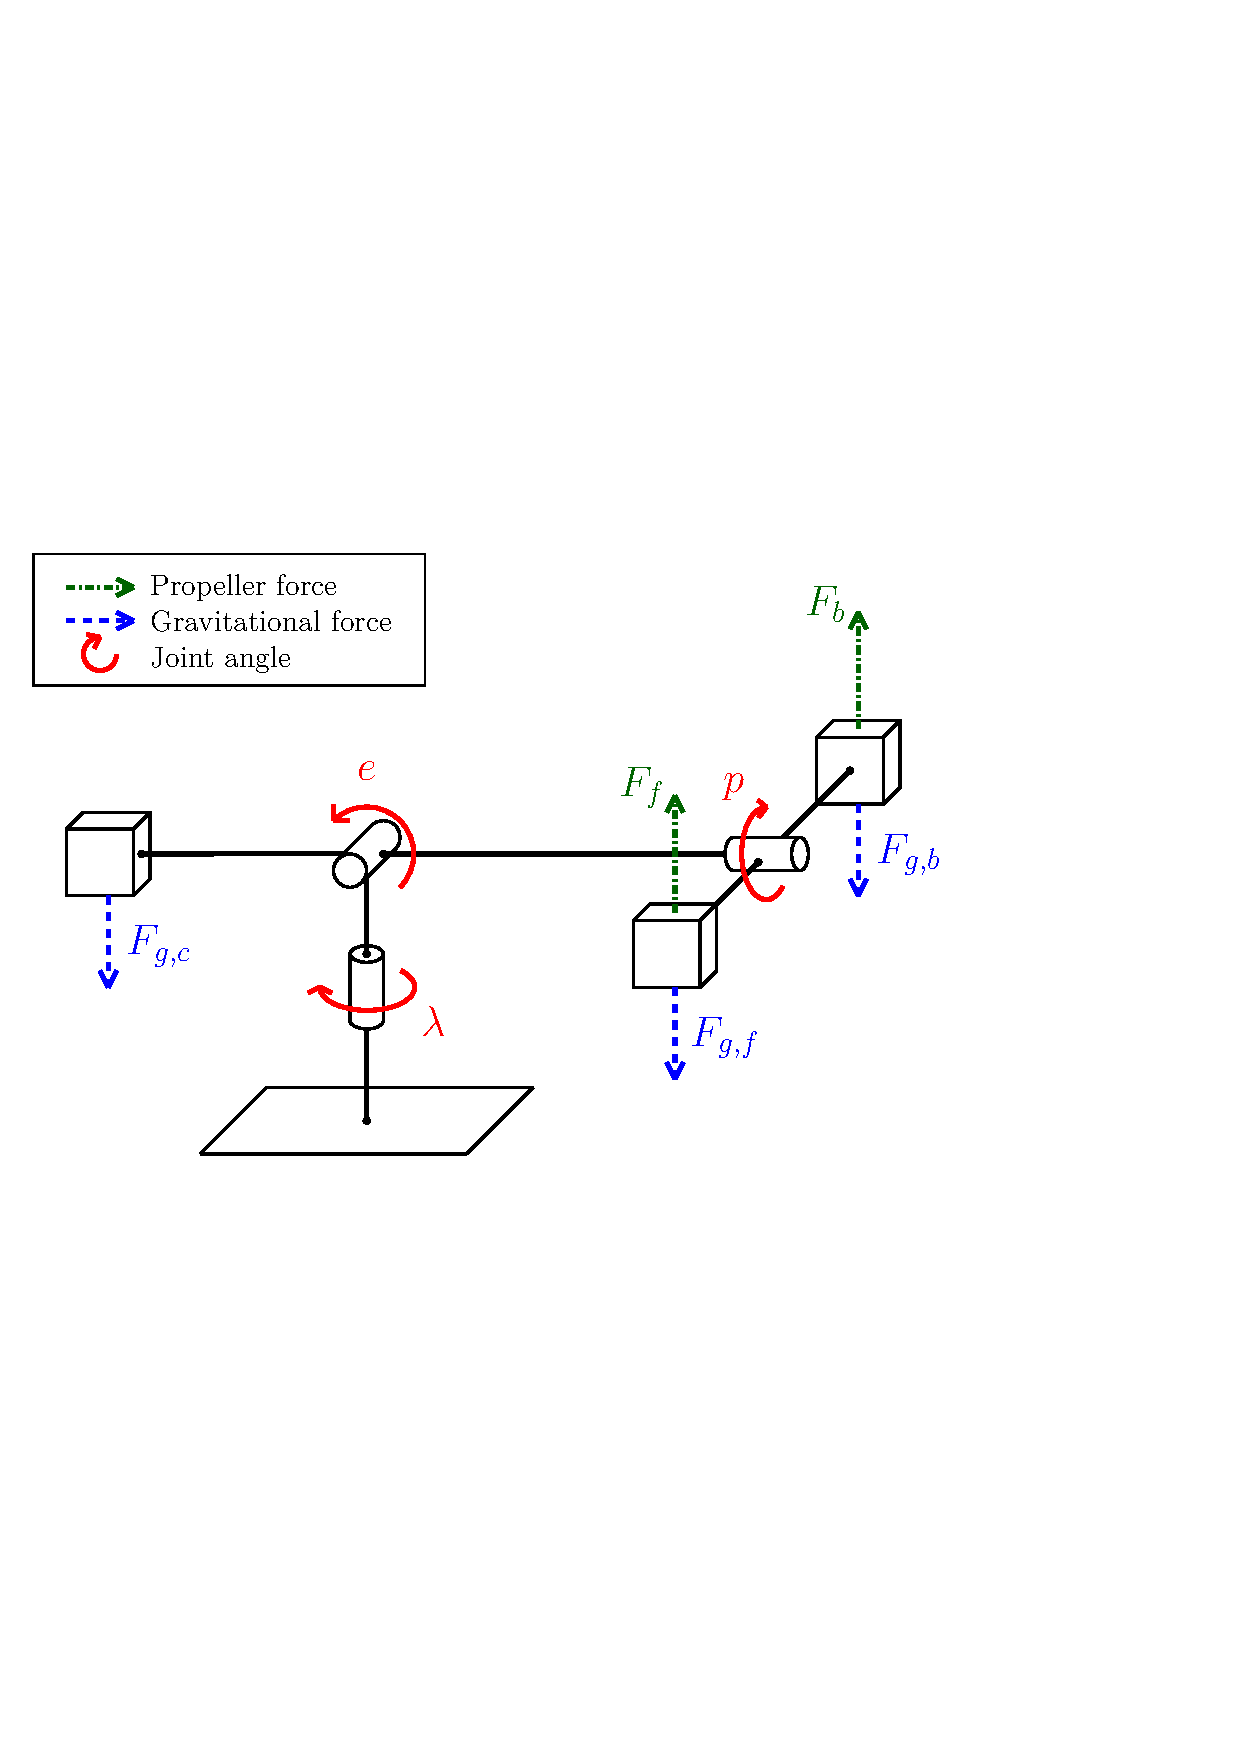
\includegraphics[width=0.80\textwidth]{figures/forces.pdf}
	\caption{Depiction of model of system.}
\label{fig:heli}
\end{figure}

The report is divided into four parts. The first part will make mathematical descriptions of the described system. Part II will describe the implementation of monovariable control through the use of PD and P controllers. Part III will describe the implementation of an LQR controller and lastly, Part IV will describe the implementation of a state estimation model into the LQR controller.

\newcommand{\texMacro}[2]{\texttt{\textbackslash{#1}\{#2\}}}
\section{General LaTeX tips}\label{sec:latex_tips}
Some tips were given in \Cref{sec:intro}, and this section will elaborate with some more concrete examples.

\subsection{Matrix Equations}
Here is a matrix equation you can use as a template:
\begin{equation}
	\begin{bmatrix}
		1 &  0 &  0 & 0 & -b &  0 &  0 &  0 \\
		-a &  1 &  0 & 0 &  0 & -b &  0 &  0 \\
		0 & -a &  1 & 0 &  0 &  0 & -b &  0 \\
		0 &  0 & -a & 1 &  0 &  0 &  0 & -b                                
	\end{bmatrix}
	\begin{bmatrix} x_1 \\ x_2 \\ x_3 \\ x_4 \\ u_0 \\ u_1 \\ u_2 \\ u_3 \end{bmatrix}
	=
	\begin{bmatrix}
		ax_0 \\ 0 \\ 0 \\ 0      
	\end{bmatrix}
\end{equation}

\subsection{Tables}
If you want, you can use the source for \Cref{tab:parameters} to see how a (floating) table is made. 

Variables and symbols are always in italics, while units are not.

\subsection{The \texMacro{input}{} command}
By using \texMacro{input}{whatever} in your main tex file (\texttt{labreport.tex} in this case), the content of \texttt{whatever.tex} will be included in your pdf. This way you can split the contents into different files, e.g.~one for each problem of the assignment. This makes it easier to restructure the document, and arguably improves the readability of the tex files. For instance; maybe you want each problem to start on a new page? Simply add \textbackslash{newpage} before each \texMacro{input}{} command. Alternatively, you can use the \texMacro{include}{} command to achieve more or less the same effect. See~\cite{InputVsInclude} for more information.

\subsection{Citations and Reference Management}
In academic writing, it is very important to cite your sources. In Latex this is done by defining an an entry in a \emph{BibTeX} bibliography file like this (from \texttt{bibliography.bib}):
\lstinputlisting[language=Tex, firstline=1, lastline=7]{bibliography.bib}
and then using the \texttt{\textbackslash{cite}} command in your Latex document. For instance \texttt{\textbackslash{cite}\{Chen2014\}} will produce~\cite{Chen2014}.

There are many different citation styles, and a lot of customization that is possible, so please check out e.g.~\cite{BiberBibtexEtc,WikibookLatex}\footnote{Keep citation of web pages to a minimum, and consider using \url{http://web.archive.org} if you are worried that the reference may change or be removed in the future.}.

There is also a lot of useful software to manage your references. Some popular examples include JabRef (\url{http://www.jabref.org/}), Mendeley (\url{https://www.mendeley.com/}) and EndNote. JabRef is perhaps the simplest of these three, and stores all information in a \texttt{.bib} file that you can directly use in your Latex document. Both Mendeley and EndNote can export references as BibTeX.

\section{Results and Figures}\label{sec:figures}
%%%%%%%%%%%%%%%%%%%%%%%%%%%%%%%%%%%%%%%%%%%%%%%%%%%%%%%%%%%%%%%%%%%%
\subsection{Part I - Mathematical modelling}\label{subsec:part1}
\subsubsection{Problem 1}

In the following derivations, Newton's 2nd law of motion for rotation is used:

\begin{equation}\label{eq:P1_N2}
    J \dot{\omega} = \sum \tau
\end{equation}
Computing the equations of motion around the pitch using~\cref{eq:P1_N2},~\cref{fig:heli} and \cref{eq:P1_forces_propellers}:
\begin{align}
    J_p \ddot{p} &= l_p F_f - l_p F_b \nonumber \\
    J_p \ddot{p} &= l_p K_f V_f - l_p K_f V_b \nonumber \\
    J_p \ddot{p} &= l_p K_f (V_f - V_b) \nonumber \\
    J_p \ddot{p} &= L_1 V_d, \quad L_1 = l_p K_f \quad V_d = V_f - V_b
    \label{eq:P1_pitch_non-linear}
\end{align}
For the elevation we also use the same procedure
\begin{align}
    J \dot{\omega} &= \sum \tau \nonumber \\
    J_e \ddot{e} &= g l_c m_c \cos{e} - 2 g l_h m_p \cos{e} + K_f l_h V_f \cos{p} + K_f l_h V_b \cos{p} \nonumber \\
    J_e \ddot{e} &= L_2 \cos{e} + L_3 V_s \cos{p}, \label{eq:P1_elevation_non-linear}\\    
                 &  \quad L_2 = g (l_c m_c - 2 l_h m_p),
                    \quad L_3 = K_f l_h,
                    \quad V_s = V_f + V_b \nonumber
\end{align}
Finally we need to calculate the travel
\begin{align}
    J \dot{\omega} &= \sum \tau \nonumber \\
    J\ddot{\lambda} &= -(K_f l_h V_f + K_f l_h V_b)\cos{e}\sin{p} \nonumber \\
    J\ddot{\lambda} &= L_4 V_s \cos{e} \sin{p},
                        \quad L_4 = - K_f l_h
                        \label{eq:P1_travel_non-linear}
\end{align}
The reason for the negative sign is because a positive pitch gives a negative travel rate. The angles are because zero pitch angle gives zero travel rate, and zero elevation angle gives maximum travel rate.

To summarise we get the following constants
\begin{subequations}\label{eq:P1_constants_for_non-linear_eq}
    \begin{align}
        L_1 &= K_f l_p \label{eq:P1_L1} \\
        L_2 &= g (l_c m_c - 2 l_h m_p) \label{eq:P1_L2} \\
        L_3 &= K_f l_h \label{eq:P1_L3} \\
        L_4 &= -K_f l_h \label{eq:P1_L4}
    \end{align}
\end{subequations}

\subsubsection{Problem 2}
In this part we wish to linearise around the point
\begin{equation*}
    \begin{bmatrix}
        p \\
        e \\
        \lambda \\
    \end{bmatrix}
    =
    \begin{bmatrix}
        p^* \\
        e^* \\
        \lambda^* \\
    \end{bmatrix}
    =
    \begin{bmatrix}
        0 \\
        0 \\
        0 \\
    \end{bmatrix}
\end{equation*}
The linearisation will be with the helicopter horizontal in both pitch and elevation. As well as no travel. For the equilibrium point $V_d^*$ and $V_s^*$ needs to be determined. It's quite easy to imagine that $V_d^*$ will be zero, as anything else would give a $\dot{p} \neq 0$.

To derive $V_s^*$ it is possible to use the equations from last problem. Specifically \ref{eq:P1_elevation_non-linear}
\begin{align*}
     J_e \ddot{e} &= L_2 \cos{e} + L_3 V_s \cos{p} \\
     J_e * 0 &= L_2 + L_3 * V_s^* \\
     V_s^* &= -\frac{L2}{L3} \\
     V_s^* &= -\frac{g(l_c m_c - 2 l_h m_p)}{K_f l_h}
\end{align*}
To summarise
\begin{subequations}
    \begin{align}
        V_s^* &= -\frac{g(l_c m_c - 2 l_h m_p)}{K_f l_h} \label{eq:P1p2_Vs} \\
        V_d^* &= 0 \label{eq:P1p2_Vd}
    \end{align}    
\end{subequations}
To simplify further analysis, the following coordinate transformation is introduced.
\begin{equation}
    \begin{bmatrix}
        \tilde{p} \\ \tilde{e} \\ \tilde{\lambda}
    \end{bmatrix}
    =
    \begin{bmatrix}
        p \\ e \\ \lambda
    \end{bmatrix}
    -
    \begin{bmatrix}
        p^* \\ e^* \\ \lambda^*
    \end{bmatrix}
    \quad \text{and} \quad
    \begin{bmatrix}
        \tilde{V}_s \\ \tilde{V}_d
    \end{bmatrix}
    =
    \begin{bmatrix}
        V_s \\ V_d
    \end{bmatrix}
    -
    \begin{bmatrix}
        V_s^* \\ V_d^*
    \end{bmatrix}
\end{equation}
Which gives the following motion equations.
\begin{equation}
    \begin{bmatrix}
        p \\ e \\ \lambda
    \end{bmatrix}
    =
    \begin{bmatrix}
        \tilde{p} \\ \tilde{e} \\ \tilde{\lambda}
    \end{bmatrix}
    \quad \text{and} \quad
    \begin{bmatrix}
        V_s \\ V_d
    \end{bmatrix}
    =
    \begin{bmatrix}
        \tilde{V}_s \\ \tilde{V}_d
    \end{bmatrix}
    +
    \begin{bmatrix}
        -\frac{L_2}{L_3} \\ 0
    \end{bmatrix}
\end{equation}
To linearise we use the Jacobian and evaluate in our equilibrium
\begin{equation}
    a_{i,j} = \frac{\del f_i}{\del x_j}
\end{equation}

%%%%%%%%%%%%%%%%%%%%%%%%%%%%%%%%%%%%%%%%%%%%%%%%%%%%%%%%%%%%%%%%%%%%
\subsection{Part II - Monovariable Control}\label{subsec:part2}
Part II takes a look at PD and P controllers. The PD is for pitch, and P for travel rate. The following formulas describe the controllers.

\begin{align}
        \tilde{V}_d &= K_{pp} (\tilde{p}_c - \tilde{p}) - K_{pd}\td{p}  \label{eq:P2_PD}\\  
        \tilde{p}_c &= K_{rp} (\td{\lambda}_c - \td{\lambda}) \label{eq:P2_P}
\end{align}

\subsubsection{Problem 1}
It is possible to derive the dynamics of \eqref{eq:P2_PD} by replacing $\tilde{V}_d$ with the linearised equation from part I, \eqref{eq:P1_lin_eq_of_motion_p}.
\begin{align*}
    \tilde{V}_d &= K_{pp} (\tilde{p}_c - \tilde{p}) - K_{pd}\td{p}) \\
    \frac{\tdd{p}}{K_1} &= K_{pp} (\tilde{p}_c - \tilde{p}) - K_{pd}\td{p}) \\
    \tdd{p} &= K_1(K_{pp}(\tilde{p}_c - \tilde{p}) - K_{pd} \td{p})
\end{align*}
If we assume initial conditions to be zero, we arrive at the following laplace transform
\begin{align}
    s^2\tilde{P} &= K_1(K_{pp}(\tilde{P}_c - \tilde{P}) - sK_{pd} \tilde{P}  \nonumber \\
    \tilde{P} &= \frac{K_1 K_{pp}}{s^2 + K_1 K_{pd} s + K_1 K_{pp}} \tilde{P}_c \nonumber \\
    H(s) &= \frac{K_1 K_{pp}}{s^2 + K_1 K_{pd} s + K_1 K_{pp}}
\end{align}
From this, the following damping ratio and natural frequency follows
\begin{align}
    \zeta &= \frac{K_1 K_{pd}}{2\sqrt{K_1 K_{pp}}} \label{eq:P2_damping_ratio} \\
    \omega_0 &= \sqrt{K_1 K_{pp}} \label{eq:P2_natural_frequency}
\end{align}
This is familiar ground. For optimal behaviour, we choose $\zeta = 1$ as this corresponds to what is known as critical damping. Which in turn means the optimal damping, where the system is neither under or over damped.\\
With $\zeta = 1$, \eqref{eq:P2_damping_ratio} and \eqref{eq:P2_natural_frequency} yields 
\begin{align}
    K_{pd} = 2\sqrt{\frac{K_{pp}}{K_1}} \label{eq:P2_Kpd} \\
    K_{pp} = \frac{\omega_0^2}{K_1}. \label{eq:P2_Kpp} 
\end{align}
Finding an optimal $\omega_0$ is difficult, but as we can see in \eqref{eq:P2_Kpd}, $K_{pd}$ is purely dependent on $K_{pp}$ and the constant $K_1$. Thus, we can tune the pitch controller simply by testing different values of $K_{pp}$.\\
\\
To systematically test different values of $K_{pp}$, we created a simple matlab script that takes the pitch from $45\degree$ to $0\degree$ and tracks the response. Using a step \textit{down} to $0\degree$ like this is a good idea since our model is linearized around that value. We test for $K_{pp}$s ranging from $4$ to $20$ all the while holding the helicopter still at 0 elevation to isolate the pitch behaviour. Our findings, shown in Figure \ref{fig:P2p1_K_pp}, show that a $K_{pp}$ of about $10$ gives a rapid response without overshoot. With the 
\begin{itemize}
    \item $K_{pp} = 10$
    \item $K_{pd} = 6.65$
\end{itemize}
\begin{figure}[!!ht!!!!!!!!tb!!]
	\centering
		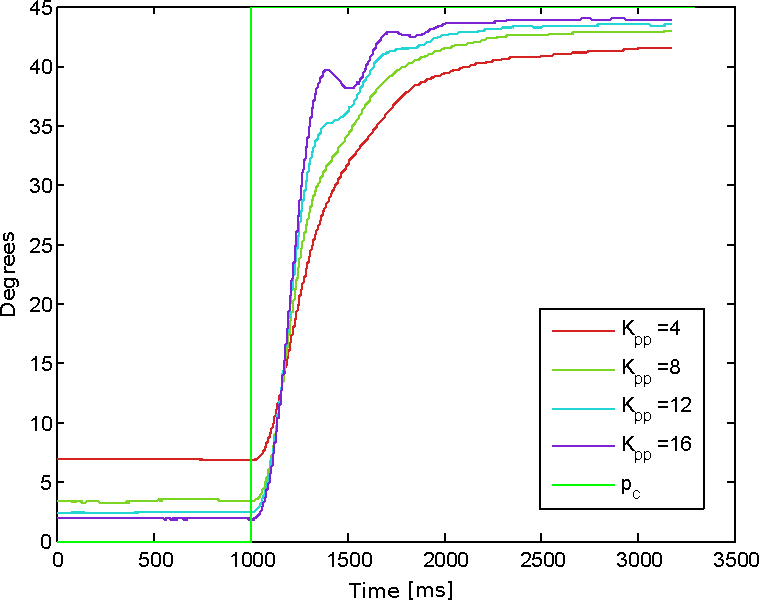
\includegraphics[width=1\textwidth,trim={0cm 0cm 0cm 0cm},clip]{figures/P2p1_K_pp_label.pdf}
	\caption{Pitch response with PD control}
\label{fig:P2p1_K_pp}
\end{figure}

\clearpage

\subsubsection{Problem 2}
The transfer function for the travel controller in \eqref{eq:P2_P} can be written as
\begin{equation}
    \frac{\td{\lambda}(s)}{\td{\lambda}_c(s)} = \frac{\rho}{s + \rho}, 
    \label{eq:P2_p_trasfer}
\end{equation}
where $\rho$ is a constant. To show this, we assume $\tilde p = \tilde p_c$ and get from \eqref{eq:P1_lin_eq_of_motion_l} that
\begin{align}
    \tilde{p} &= \frac{\tdd{\lambda}}{K_3} \label{eq:P2_p_to_lambda}.
\end{align}
Inserting this into \eqref{eq:P2_P} then yields
\begin{align*}
    \tdd{\lambda} &= K_3 K_{rp} (\td{\lambda}_c - \td{\lambda}),
\end{align*}
which in the laplace domain is
\begin{align*}
    s\td{\lambda} &= K_3 K_{rp} (\td{\lambda}_c - \td{\lambda}).
\end{align*}
Finally, by rearranging the terms, we get the transfer function 
\begin{align}
    h(s) = \frac{\td{\lambda}}{\td{\lambda}_c} = \frac{K_3 K_{rp}}{s + K_3 K_{rp}},
\end{align}
which when letting $\rho = K_3 K_{rp}$ becomes \eqref{eq:P2_p_trasfer}.
\begin{figure}[!!ht!!!!!!!!tb!!]
	\centering
		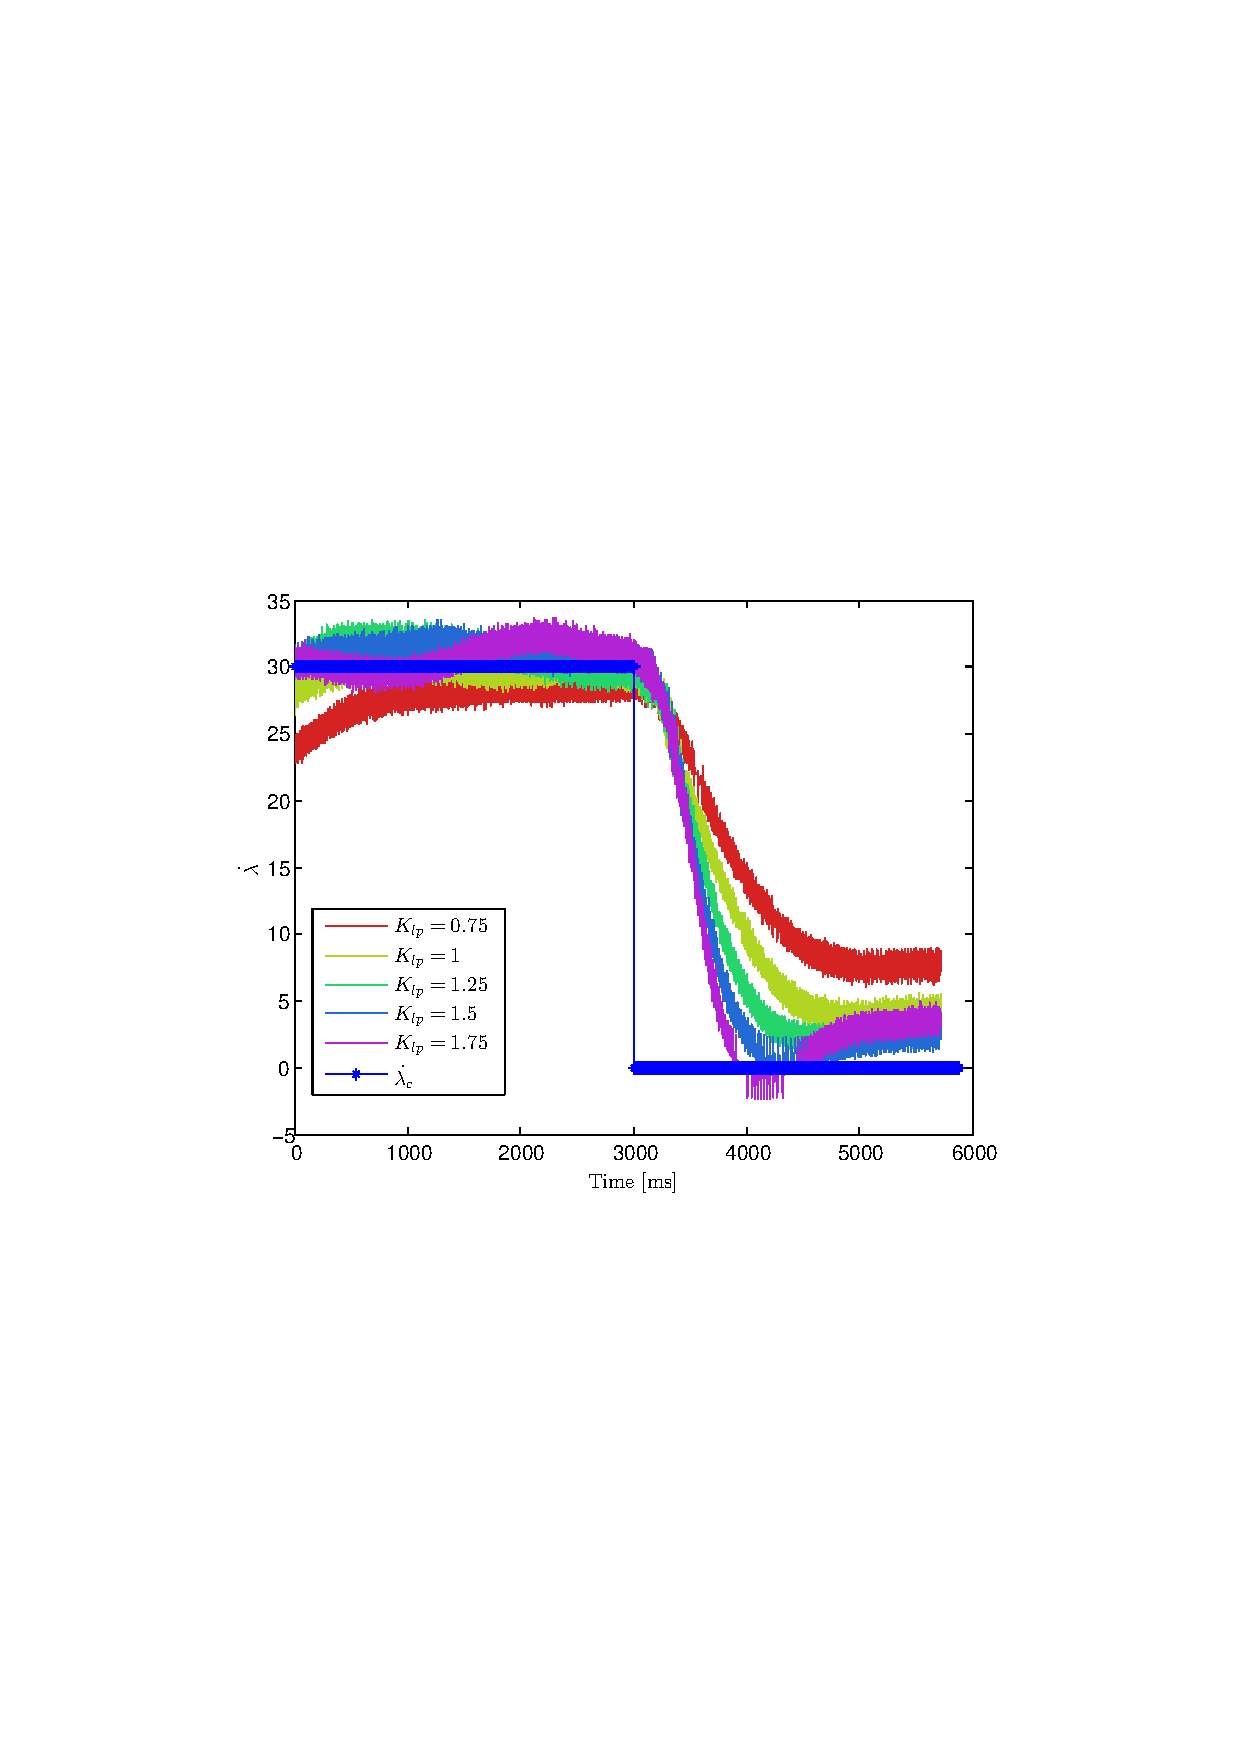
\includegraphics[width=1\textwidth,trim={4cm 9cm 4cm 9cm},clip]{figures/P2p2_Klp.pdf}
	\caption{Travel response with P control}
\label{fig:P2p2_K_lp}
\end{figure}
\clearpage
%%%%%%%%%%%%%%%%%%%%%%%%%%%%%%%%%%%%%%%%%%%%%%%%%%%%%%%%%%%%%%%%%%%%
\subsection{Part III - Multivariable control}



We don't need reference feed forward (P matrix) (F matrix???) when using integral effect. So we can use the same P matrix as in the previous problem. Sources on wikipendium and in Chen (Chapter 9 problem solutions 9.4).
\subsubsection{Problem 1}


Considering~\cref{eq:P1_lin_eq_of_motion} and a state vector and input of  

\begin{equation}\label{P3_state_vector_and_input}
    \mathbf{x}=
    \begin{bmatrix}
        \tilde{p}\\
        \td{p}\\
        \td{e}
    \end{bmatrix}
    \quad\text{and}\quad
    \mathbf{u}=
    \begin{bmatrix}
        \tilde{V_s}\\
        \tilde{V_d}
    \end{bmatrix}
\end{equation}

and a state-space formulation of the form
\begin{equation}\label{eq:P3_state_space_equation}
    \dot{\mathbf{x}}=\mathbf{Ax}+\mathbf{Bu}    
\end{equation}

the matrices $\mathbf{A}$ and $\mathbf{B}$ are given by 

\begin{subequations}\label{eq:P3_p1_A_B}
    \begin{align}
        \mathbf{A}=
            \begin{bmatrix}
                0&1&0\\
                0&0&0\\
                0&0&0
            \end{bmatrix}\label{eq:P3_p1_A} \\
        \mathbf{B}=
            \begin{bmatrix}
                0&0\\
                K_1&0\\
                0&K_2
            \end{bmatrix}\label{eq:P3_p1_B}.
    \end{align}
\end{subequations}

\subsubsection{Problem 2}

For this problem, the purpose was to track a reference

\begin{equation}\label{eq:P3_p2_reference}
    \mathbf{r}=
        \begin{bmatrix}
            \tilde{p_c}\\
            \dot{\tilde{e_c}}
        \end{bmatrix}
\end{equation}

Firstly, the controllability of the system is examined. Due to having three states, the controllability matrix is given by

\begin{equation}\label{eq:P3_p2_controllability_matrix}
    \mathcal{C}=
        \begin{bmatrix}
            \mathbf{B}&\mathbf{AB}&\mathbf{A^2B}
        \end{bmatrix}
\end{equation}

Using $K_1=0.9046$ and $K_2=0.1555$, the controllability matrix is given by

\begin{equation}
    \mathcal{C}=
        \begin{bmatrix}
            
        \end{bmatrix}
\end{equation}

Calculating the controllability matrix with 

\begin{figure}[!!ht!!!!!!!!tb!!]
	\centering
		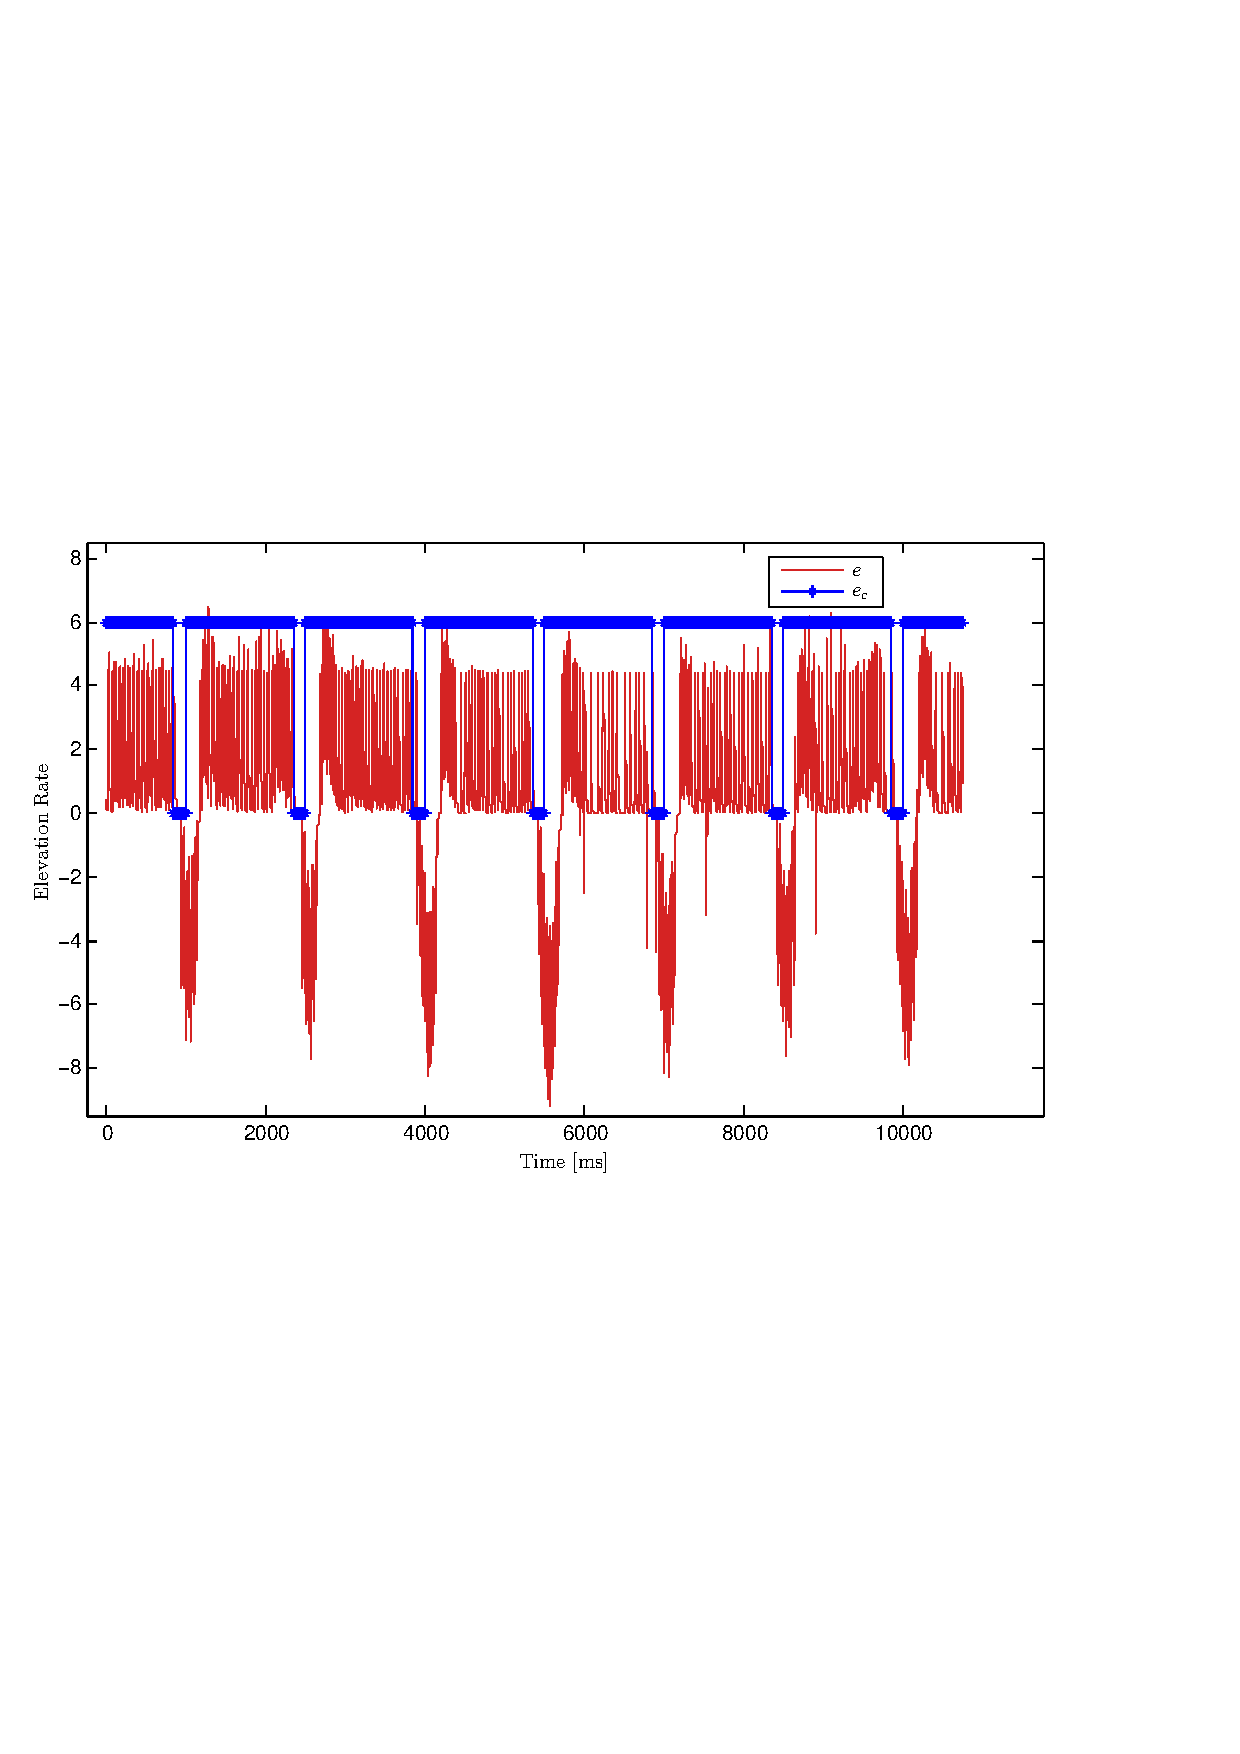
\includegraphics[width=1\textwidth,trim={4cm 9cm 4cm 9cm},clip]{figures/P3p2_e_dot.pdf}
	\caption{Travel response with P control}
\label{fig:P3p2_e_dot}
\end{figure}
\clearpage
\begin{figure}[!!ht!!!!!!!!tb!!]
	\centering
		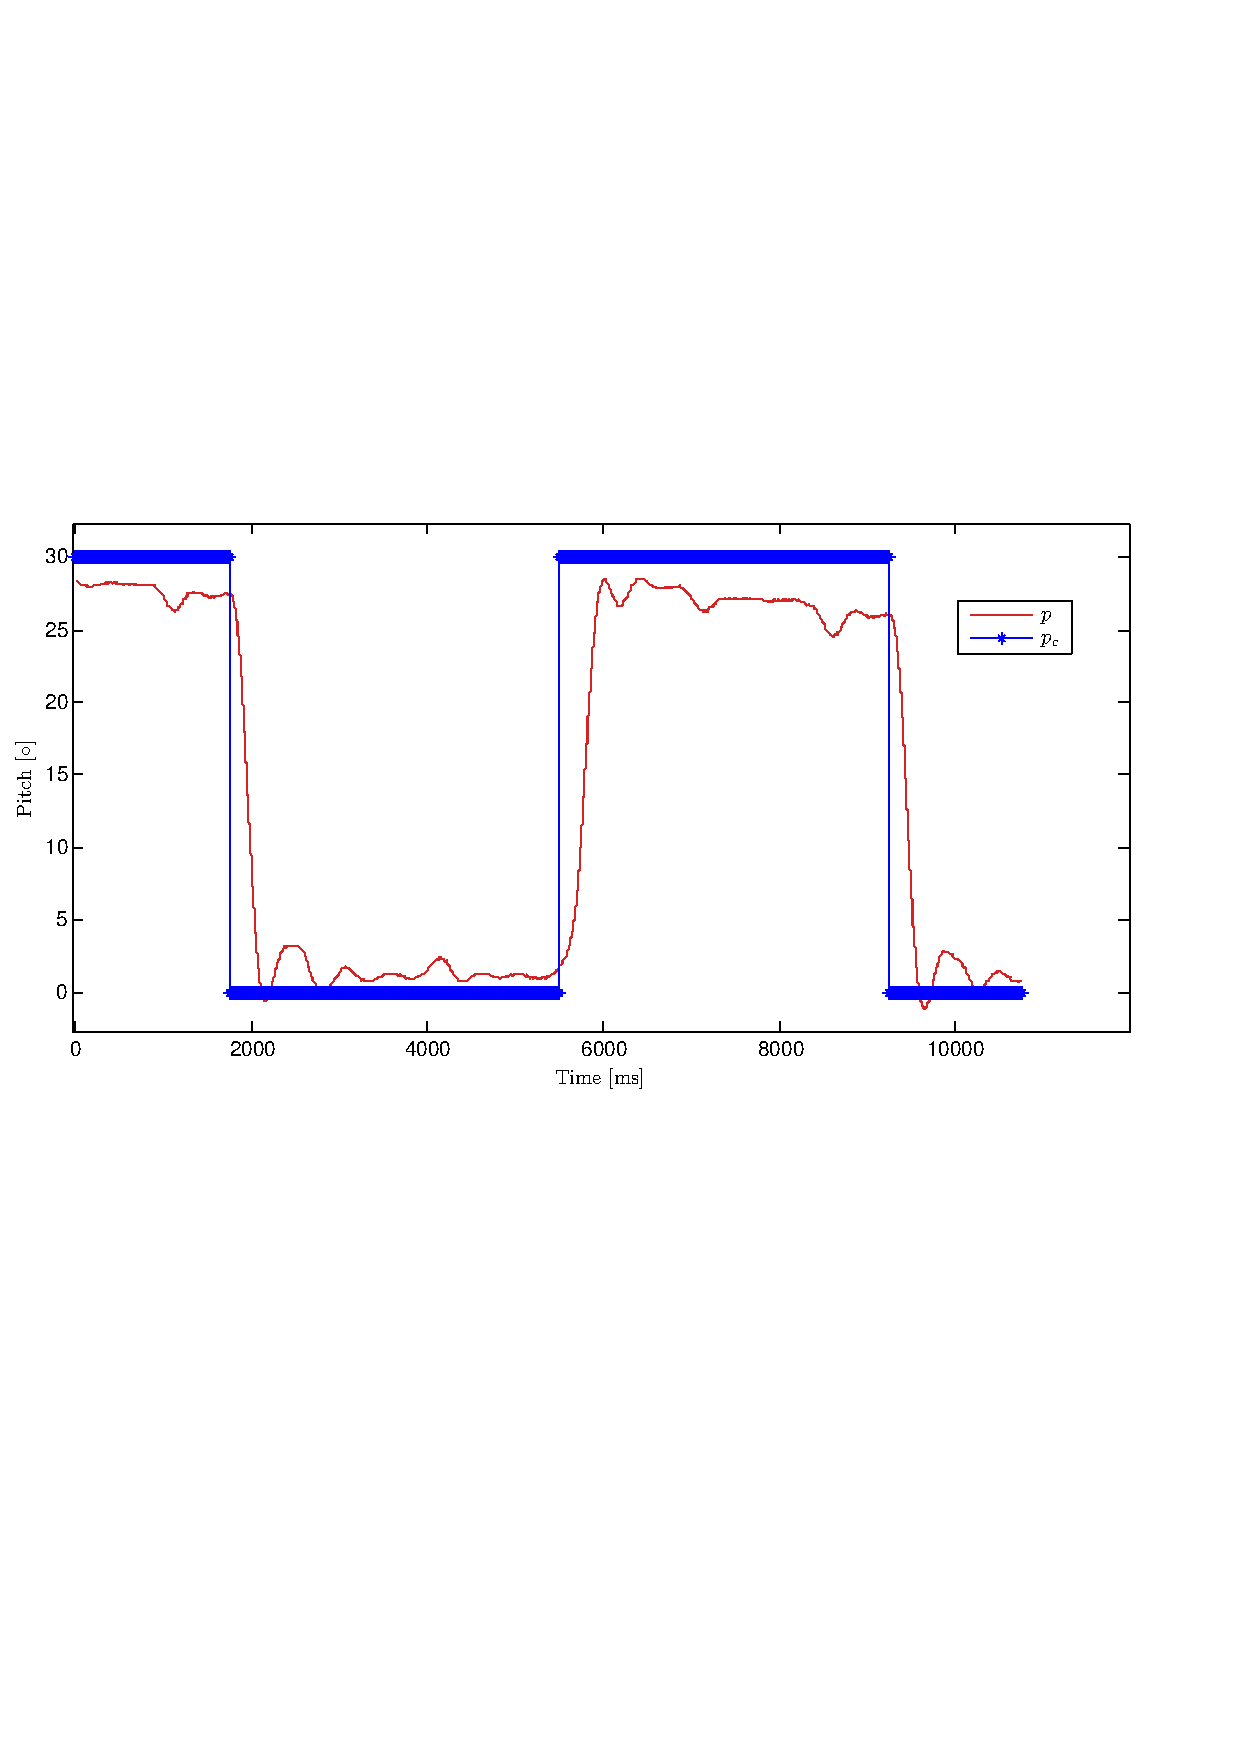
\includegraphics[width=1\textwidth,trim={4cm 9cm 4cm 9cm},clip]{figures/P3p2_p.pdf}
	\caption{Travel response with P control}
\label{fig:P3p2_p}
\end{figure}
\clearpage
%%%%%%%%%%%%%%%%%%%%%%%%%%%%%%%%%%%%%%%%%%%%%%%%%%%%%%%%%%%%%%%%%%%%
\subsection{Part IV - State estimation}









Answer all the parts of the exercise in an organized and clear manner. You should of course try to get good results in all the exercises, but if you have made a good effort without achieving great performance, a good discussion of possible reasons is just as good. Present your thinking and efforts and discuss possible reasons for good or bad results.

Include plots and/or tables of all relevant results, but make sure you don't overwhelm the reader with too many plots. Have a clear plan about what you want to communicate with a specific plot/figure, and use appropriate labels and comments. Keep in mind that the plots should be as ``readable'' as possible; that is, they should not be too hard to interpret and be reasonably self contained.

There are some important things to consider when exporting figures from MATLAB, most importantly which format you use. Always ever use JPEG for anything that is not a photography or similar. Any figure, like a plot or block diagram, must be stored as a JPEG\@. If you zoom in on \Cref{fig:constraint_jpg} you can see a lot of beauty close to any of the dark curves and lines, this is due to the lovely nature of JPEG\@. \Cref{fig:constraint_jpg} will look fantastic both on a screen and on paper.

The PNG format is slightly better for plots, but since it is a raster format (a grid of pixels), it looks ugly if you zoom in. It also looks ugly if you scale it, both on a screen and on paper. Try to avoid PNG if you can. \Cref{fig:constraint_png,fig:constraint_png_large} are both PNG figures; the latter being a larger figure scaled more than the former. Note both how choppy and ugly the blue curve is, and how the different sizes create inconsistent font sizes.

The simplest way to get a reasonably good looking plot is to save it as EPS in MATLAB\@. Do this by clicking ``File'' in the figure window, and the ``Save As\ldots''; choose ``EPS file (*.eps)'' in the ``Save as type:'' menu.\footnote{pdfLatex does not support EPS directly, but since we have loaded the \emph{epstodf} package, this is not a problem.} \Cref{fig:constraint_eps} shows a plot in EPS format. Since EPS is a vector format, the Figure can be scaled and still look good (but mind the font size!). If you zoom in you can see that the curve and the letters/numbers are smooth. A figure in vector format will usually look good both on a screen and on paper.

Note that the size of the actual figure window in MATLAB determines how large the exported figure is. Hence, if you enlarge the figure window before exporting, you will need to scale the figure by a larger factor in the report. This will lead to a tiny font in the figure. There are many better ways of exporting graphics from MATLAB, but they quickly become fairly involved. The above method of exporting to EPS will in most cases give nice figures.

You can write Latex in your MATLAB figures. The script used to create \Cref{fig:constraint_jpg,fig:constraint_eps} is included in \Cref{sec:plot_constraint_m}. Do not use a screen shot of a scope of figure in MATLAB in your report.


\begin{figure}[htb]
	\centering
		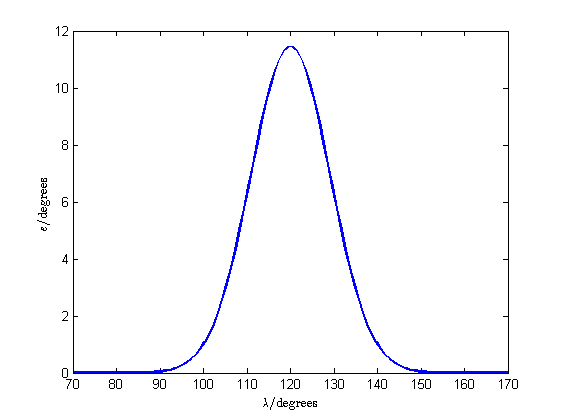
\includegraphics[width=0.8\textwidth]{figures/constraint_png.png}
	\caption{A plot in PNG format --- a bad idea.}
\label{fig:constraint_png}
\end{figure}

\begin{figure}[htb]
	\centering
		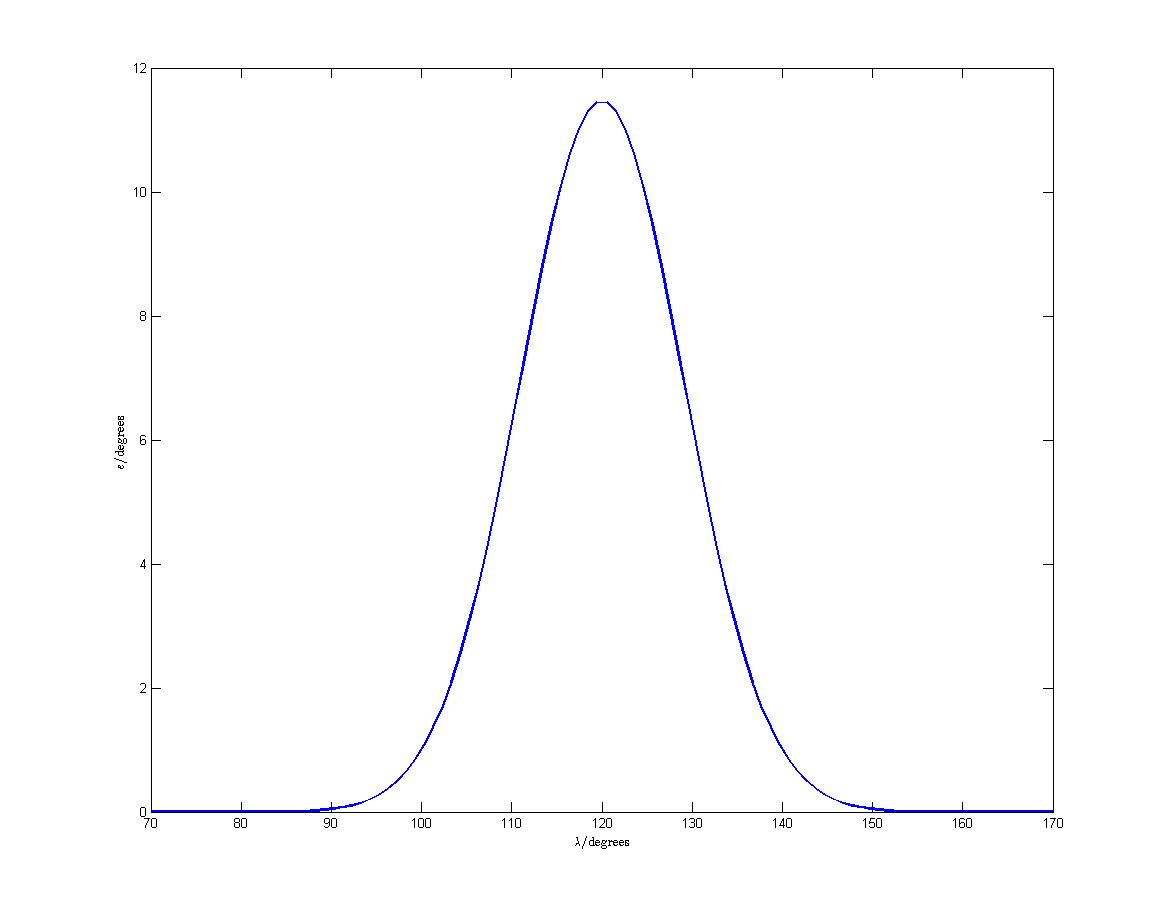
\includegraphics[width=0.8\textwidth]{figures/constraint_png_large.png}
	\caption{A plot in PNG format --- a bad idea. This figure is originally larger than the other PNG figure, but both are scaled to the same size.}
\label{fig:constraint_png_large}
\end{figure}

\begin{figure}[htb]
	\centering
		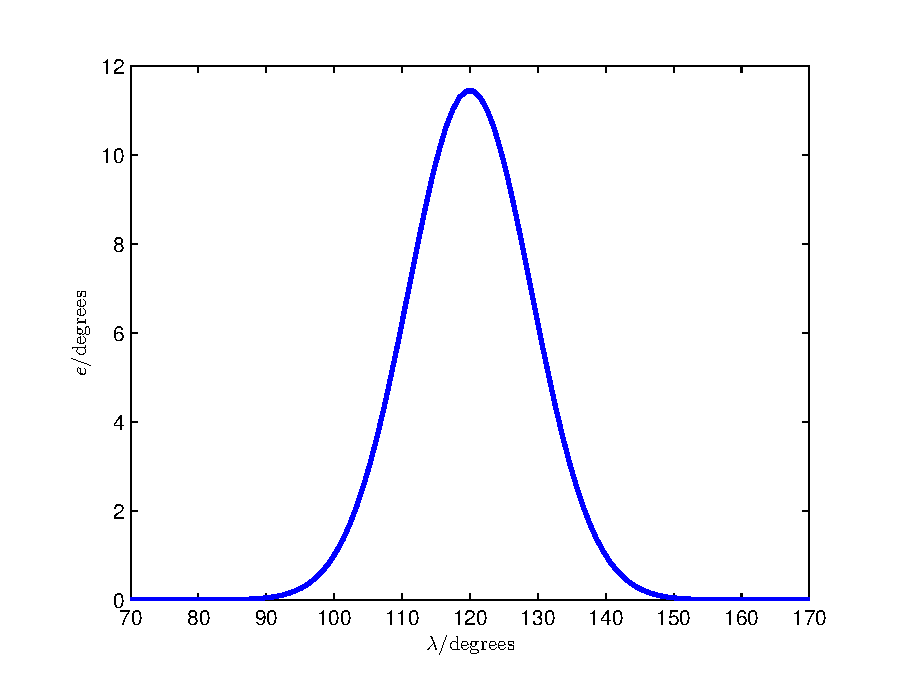
\includegraphics[width=0.8\textwidth]{figures/constraint_eps.eps}
	\caption{A plot in EPS format --- a much better idea.}
\label{fig:constraint_eps}
\end{figure}

Remember to reference all figures in the text. Figures have a number and should be referenced by that number (again, always use dynamic references). They also tend to float around, meaning they generally don't appear where you ask them to in the text. This is fine, do not try to force a figure (or a table) to appear in a particular place. As long a you refer to it, it's easy to find. No figure should be included without being referenced in the text.

If you look at the source code for including figures, you can see that the optional option \verb+[htb]+ has been used. This tells Latex where you wish the figure to appear, in prioritized order. \verb+h+ means ``Here'', t means ``Top of this page'', b means ``Bottom of this page'', and p (not used here) means ``on a Page with only floats (such as figures and tables)''. Note that your wish might not be granted, and this is because Latex actually optimizes the placement of figures. If you start forcing figures to be in specific places, it often leads to really strange layout somewhere else in the document. 

Generally, let Latex handle the documentation layout. This is one of the main reasons to choose Latex over software such as Microsoft Word.

\subsection{Results and Discussion}
All problems should have their own discussion of results. 

Remember: all plots and results need a description, explanation, and discussion.

\include{part4}
\section{Problems}\label{sec:problems}
\subsection{Part IV}
\subsubsection{Problem 1}
The system given in the equations (TODO: ADD REFERENCE) can be expressed as a state space equation 
with the vectors
\begin{align}
    \textbf{x} = \begin{bmatrix}
        \tilde p        \\
        \td p           \\
        \tilde e        \\
        \td e           \\
        \tilde \lambda  \\
        \td \lambda
    \end{bmatrix}, \hspace{0.5cm}
    \mathbf{u} = \begin{bmatrix}
        \tilde V_s \\
        \tilde V_d
    \end{bmatrix} \hspace{0.5cm} \text{and} \hspace{0.5cm}
    \textbf{y} = \begin{bmatrix}
        \tilde p        \\
        \tilde e        \\
        \tilde \lambda  \\
    \end{bmatrix}
\end{align}.
The equation can thus be expressed on the form
\begin{align}
    \mathbf{\dot x} &= \mathbf{Ax} + \mathbf{B} \\
    \mathbf{y} &= \mathbf{Cx},
\end{align}
with the matrices
\begin{equation}
    \setstackgap{L}{1.1\baselineskip}
    \fixTABwidth{T}
    \label{p4_sys_AB}
    \mathbf A = 
    \parenMatrixstack{
		0   & 1 & 0 & 0 & 0 & 0 \\
		0   & 0 & 0 & 0 & 0 & 0 \\
		0   & 0 & 0 & 1 & 0 & 0 \\
		0   & 0 & 0 & 0 & 0 & 0 \\
		0   & 0 & 0 & 0 & 0 & 1 \\
		K_3 & 0 & 0 & 0 & 0 & 0 
	}
	\text{,}
	\hspace{0.5cm}
	\mathbf B = 
	\parenMatrixstack{
	    0   & 0   \\
	    0   & K_1 \\
	    0   & 0 & \\
	    K_2 & 0   \\
	    0   & 0   \\
	    0   & 0
	}
\end{equation}
and
\begin{equation}
    \label{p4_sys_C}
    \mathbf C = 
    \begin{pmatrix}
        1   &   0   &   0   &   0   &   0   &   0 \\
        0   &   0   &   1   &   0   &   0   &   0 \\
        0   &   0   &   0   &   0   &   1   &   0
    \end{pmatrix}
\end{equation}.
\subsubsection{Problem 2}
From the system matrix in \eqref{p4_sys_AB} and the output matrix in \eqref{p4_sys_C}, the observability matrix can be found to be
\begin{equation}
    \setstackgap{L}{1.1\baselineskip}
    \fixTABwidth{T}
    \mathbf{\mathcal{O}} = 
        \begin{pmatrix}
        \mathbf{C}      \\
        \mathbf{CA}     \\
        \mathbf{CA^2}   \\
        \mathbf{CA^3}   \\
        \mathbf{CA^4}   \\
        \mathbf{CA^5}   \\
    \end{pmatrix}
    =
    \parenMatrixstack{
    1       & 0       & 0 & 0 & 0 & 0 \\
    0       & 0       & 1 & 0 & 0 & 0 \\
    0       & 0       & 0 & 0 & 1 & 0 \\
    0       & 1       & 0 & 1 & 0 & 0 \\
    0       & 0       & 0 & 0 & 0 & 1 \\
    0       & 0       & 0 & 0 & 0 & 0 \\
    0       & 0       & 0 & 0 & 0 & 0 \\
    -0.6117 & 0       & 0 & 0 & 0 & 0 \\
    0       & 0       & 0 & 0 & 0 & 0 \\
    0       & 0       & 0 & 0 & 0 & 0 \\
    0       & -0.6117 & 0 & 0 & 0 & 0 \\
    0       & 0       & 0 & 0 & 0 & 0 \\
    0       & 0       & 0 & 0 & 0 & 0 \\
    0       & 0       & 0 & 0 & 0 & 0 \\
    0       & 0       & 0 & 0 & 0 & 0 \\
    0       & 0       & 0 & 0 & 0 & 0 \\
    0       & 0       & 0 & 0 & 0 & 0 }
    \text{.}
\end{equation}
We note that $\mathbf{\mathcal{O}}$ has full column rank, which means the system is observable.\\
\\
We wish to control the system using an estimated state $\mathbf{\hat{x}}$. A \textit{linear observer} (or closed-loop estimator) is then
\begin{equation}
    \mathbf{\dot{\hat{x}}} = \mathbf{A\hat{x}} + \mathbf{Bu} + \mathbf{L} (\mathbf{y} - \mathbf{C\hat{x}})
\end{equation}
where $\mathbf A$, $\mathbf B$ and $\mathbf C$ are as before and $\mathbf L$ is the \textit{observer gain matrix}.

\subsubsection{Problem 3}
The matrices 
\begin{equation}
    \mathbf{C}_{e\lambda} = \begin{pmatrix}
    0 & 0 & 1 & 0 & 0 & 0 \\
    0 & 0 & 0 & 0 & 1 & 0
    \end{pmatrix}
    \quad \text{and} \quad
    \mathbf{C}_{pe} = \begin{pmatrix}
    1 & 0 & 0 & 0 & 0 & 0 \\
    0 & 0 & 1 & 0 & 0 & 0
    \end{pmatrix}
\end{equation}
correspond to the measurement vectors
\begin{equation}
    \mathbf{y}_{e\lambda} = \begin{bmatrix}
        \tilde e \\
        \tilde \lambda
    \end{bmatrix}
    \quad \text{and} \quad
    \mathbf{y}_{pe} = \begin{bmatrix}
        \tilde p \\
        \tilde e 
    \end{bmatrix}
\end{equation}
respectively.\\
Since
\begin{equation}
    \setstackgap{L}{1.1\baselineskip}
    \fixTABwidth{T}
    \mathbf{\mathcal{O}}_{e\lambda} = 
        \begin{pmatrix}
        \mathbf{C}_{e\lambda}               \\
        \mathbf{C}_{e\lambda}\mathbf{A}     \\
        \mathbf{C}_{e\lambda}\mathbf{A^2}   \\
        \mathbf{C}_{e\lambda}\mathbf{A^3}   \\
        \mathbf{C}_{e\lambda}\mathbf{A^4}   \\
    \end{pmatrix}
    = \parenMatrixstack{
    0       & 0       & 1 & 0 & 0 & 0 \\
    0       & 0       & 0 & 0 & 1 & 0 \\
    0       & 0       & 0 & 1 & 0 & 0 \\
    0       & 0       & 0 & 0 & 0 & 1 \\
    0       & 0       & 0 & 0 & 0 & 0 \\
    -0.6117 & 0       & 0 & 0 & 0 & 0 \\
    0       & 0       & 0 & 0 & 0 & 0 \\
    0       & -0.6117 & 0 & 0 & 0 & 0 \\
    0       & 0       & 0 & 0 & 0 & 0 \\
    0       & 0       & 0 & 0 & 0 & 0 \\
    0       & 0       & 0 & 0 & 0 & 0 \\
    0       & 0       & 0 & 0 & 0 & 0 }
\end{equation}
has full column rank, the system is observable when measuring only $\tilde e$ and $\tilde \lambda$. On the other hand, when measuring only $\tilde p$ and $\tilde e$, the system is \textit{not} observable, as

\begin{equation}
    \mathbf{\mathcal{O}}_{pe} = 
        \begin{pmatrix}
        \mathbf{C}_{pe}               \\
        \mathbf{C}_{pe}\mathbf{A}     \\
        \mathbf{C}_{pe}\mathbf{A^2}   \\
        \mathbf{C}_{pe}\mathbf{A^3}   \\
        \mathbf{C}_{pe}\mathbf{A^4}   \\
    \end{pmatrix}
    = \begin{pmatrix}
    1 & 0 & 0 & 0 & 0 & 0 \\
    0 & 0 & 1 & 0 & 0 & 0 \\
    0 & 1 & 0 & 0 & 0 & 0 \\
    0 & 0 & 0 & 1 & 0 & 0 \\
    0 & 0 & 0 & 0 & 0 & 0 \\
    0 & 0 & 0 & 0 & 0 & 0 \\
    0 & 0 & 0 & 0 & 0 & 0 \\
    0 & 0 & 0 & 0 & 0 & 0 \\
    0 & 0 & 0 & 0 & 0 & 0 \\
    0 & 0 & 0 & 0 & 0 & 0 \\
    0 & 0 & 0 & 0 & 0 & 0 \\
    0 & 0 & 0 & 0 & 0 & 0 \\
    \end{pmatrix}
\end{equation}
does \textit{not} have full column rank.\\
This also makes intuitive sense, as we cannot expect to observe the travel, $\lambda$, from only knowing elevation $e$ and the pitch $p$. But if we do know the travel, the pitch can be obtained by taking the derivative.  


\section{Conclusion}\label{sec:conclusion}
This does not have to be long, but try to write a few reasonable closing remarks.

\addcontentsline{toc}{section}{Appendix} % Remove this if you don't want the appendix included in the table of contents.
\appendix

\section{MATLAB Code}\label{sec:matlab}
This section should contain your MATLAB code. DO NOT attach files posted online (that you didn't write). Note that the method used to input code below does not look as pretty when the lines are too long.

\subsection{plot\_constraint.m}\label{sec:plot_constraint_m}
\lstinputlisting{code/plot_constraint.m}\section{Simulink Diagrams}\label{sec:simulink}
This section should contain your Simulink diagrams. Just like the plots, these should be in vector format, like in \Cref{fig:simulink}. Make them tidy enough to understand.

\subsection{Simulink Diagrams for Part II}
\begin{figure}[!!ht!!!!!!!!tb!!]
    	\centering
		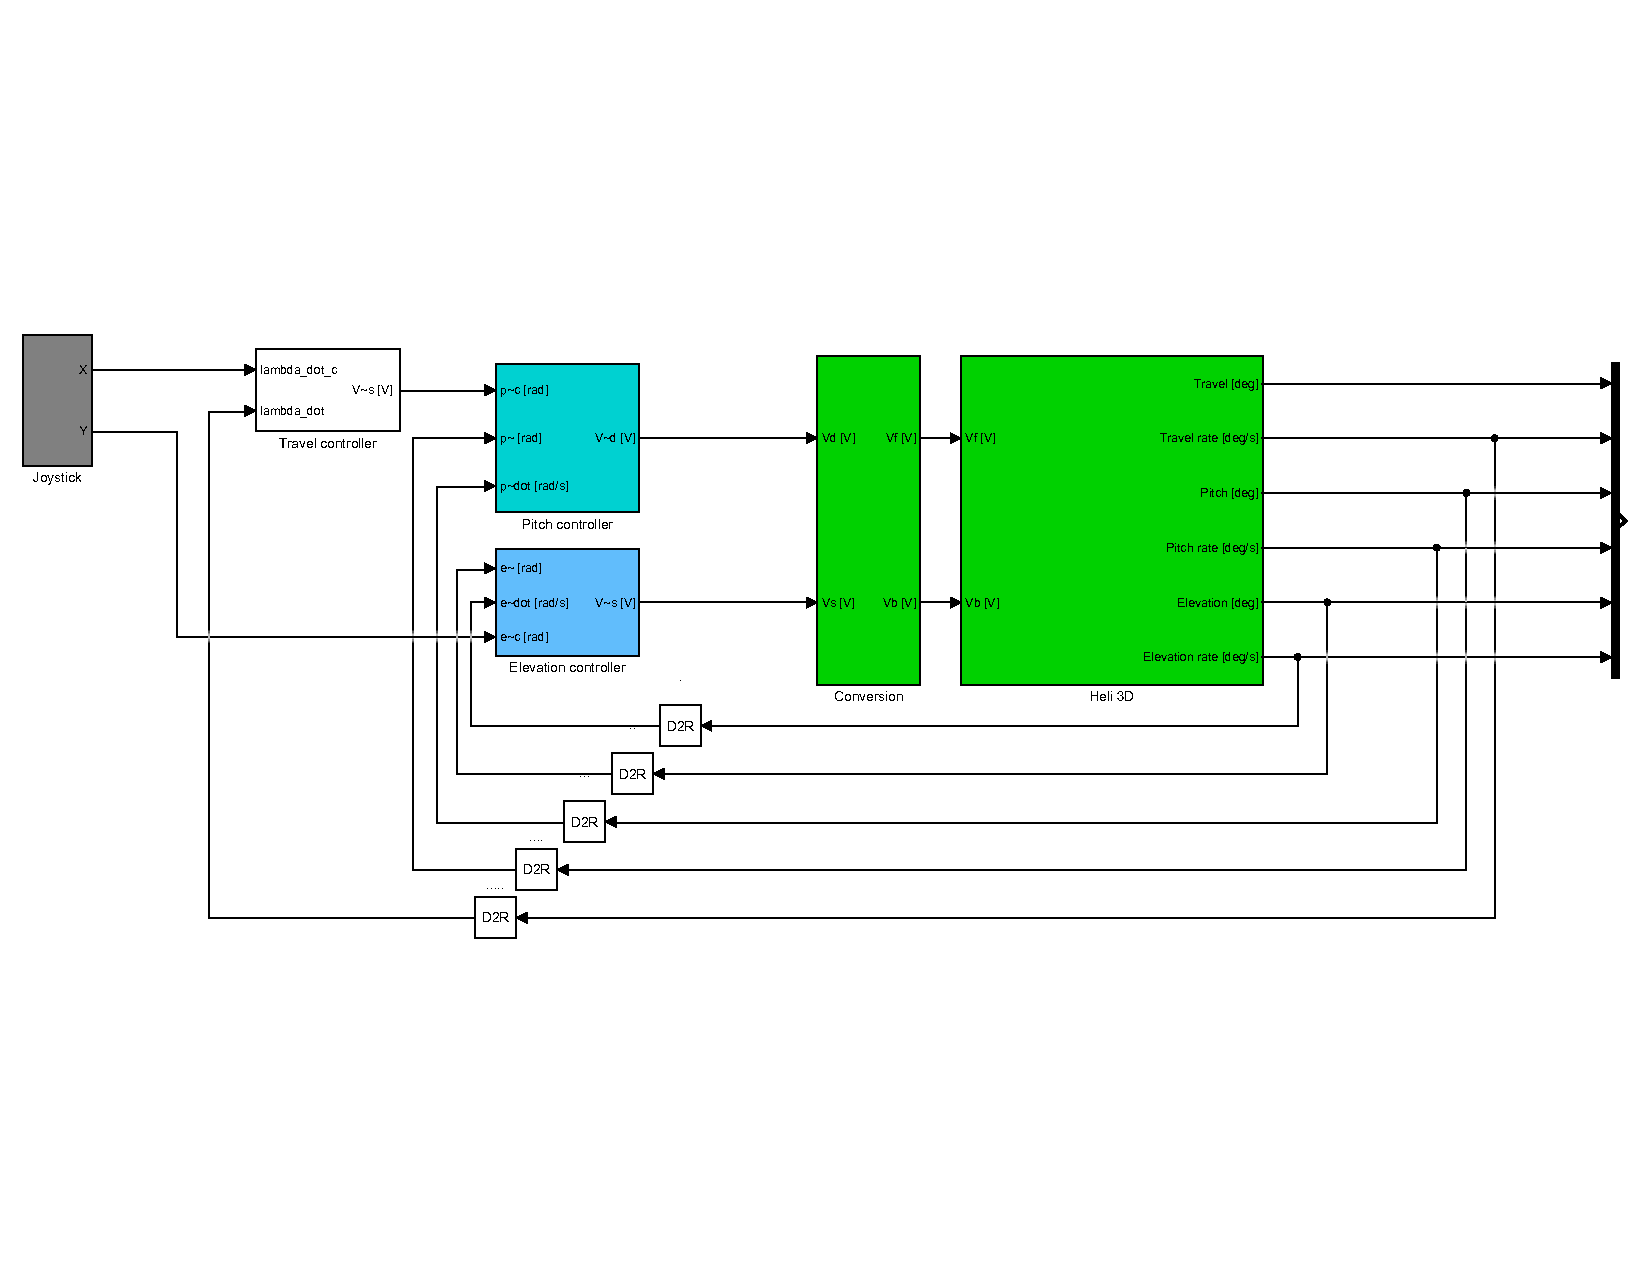
\includegraphics[width=1.1\textwidth,trim={0cm 3cm 0cm 5cm},clip]{figures/simulink/P2p2.pdf}
    	\caption{Top view of model from Part 2 problem 2}
\label{fig:P2p2_simulink}
\end{figure}
\FloatBarrier

\section{Parameters and values}\label{sec:parameters}


\begin{table}[tbp]
	\centering
	\caption{Parameters and values.}
	\begin{tabular}{llll}
		\toprule
		Symbol & Parameter & Value & Unit \\
		\midrule
		$l_h$ & Distance from elevation axis to helicopter body & $0.63$  & \meter                      \\
		$l_p$ & Distance from pitch axis to motor               & $0.18$  & \meter                      \\
		$K_f$ & Force constant motor                            & $0.25$  & \newton\per\volt            \\
		$J_e$ & Moment of inertia for elevation                 & $0.83$  & \kilogram\usk\meter\squared \\
$J_{\lambda}$ & Moment of inertia for travel                    & $0.83$  & \kilogram\usk\meter\squared \\
		$J_p$ & Moment of inertia for pitch                     & $0.034$ & \kilogram\usk\meter\squared \\
		$m_p$ & Mass of helicopter                              & $1.05$  & \kilogram                   \\
		$m_c$ & Weight of counterweight                         & $1.87$  & \kilogram                   \\
		\bottomrule
	\end{tabular}
\label{tab:parameters}
\end{table}

% \input simply inserts the contents of the file, while \include forces a \newpage.
% See \input vs. \include: http://tex.stackexchange.com/questions/246/when-should-i-use-input-vs-include

% References
\newpage
\addcontentsline{toc}{section}{References}
\printbibliography{}
\label{sec:bibliography}

\end{document}
